\documentclass[14pt,a4paper]{extarticle}%
\usepackage{amsthm}
\usepackage{amsmath}
\usepackage{amsfonts}
\usepackage{amssymb}
\usepackage{setspace}
\usepackage{listings}
\usepackage{graphicx}
\usepackage{indentfirst}
\usepackage{booktabs}
\usepackage{float}
\usepackage{longtable}
\usepackage[normalem]{ulem}
\usepackage[T2A]{fontenc}
\usepackage[utf8]{inputenc}
\usepackage[english,russian]{babel}
%-------------------------------------------
\setlength{\textwidth}{7.0in}
\setlength{\oddsidemargin}{-0.35in}
\setlength{\topmargin}{-0.5in}
\setlength{\textheight}{9.0in}
\setlength{\parindent}{0.3in}
\graphicspath{{../plot/}}


\newtheorem{theorem}{Theorem}
\newtheorem{task}[theorem]{Задача}
\addto\captionsrussian{\renewcommand*{\proofname}{Решение}}

\onehalfspacing


\begin{document}

\begin{titlepage}
  \begin{center}
    МИНОБРНАУКИ РОССИИ\\
    САНКТ-ПЕТЕРБУРГСКИЙ ГОСУДАРСТВЕННЫЙ\\
    ЭЛЕКТРОТЕХНИЧЕСКИЙ УНИВЕРСИТЕТ\\
    <<ЛЭТИ>> ИМ. В. И. ЛЕНИНА (УЛЬЯНОВА)\\
    Кафедра МО ЭВМ

    \vspace{4cm}

    ОТЧЕТ\\
    по практической работе №4\\
    по дисциплине <<Теория принятия решений>>\\
    Тема: Индикаторы технического анализа
    \vfill

    \begin{tabular}{ c c c }
      Студент гр. 8303 & \uline{\hspace{3cm}} & Гришин К. И. \\[1cm]
      Преподаватель    & \uline{\hspace{3cm}} & Попова Е. В. \\
    \end{tabular}
    
    \vfill
    Санкт-Петербург\\
    2022
  \end{center}
\end{titlepage}


\section{Цель работы}
Используя индикаторы технического анализа и инструментальные
средства смоделировать задачи принятия решений на спотовом рынке.

\section{Основные теоретические положения}
Скользящее среднее (Moving Average, MA) используется как
самостоятельный индикатор.

Сигналы на покупку поступают, когда цена актива пробивает вверх MA.

Сигналы на продажу подаются, когда цена пробивает вниз MA.

\vspace{.5cm}

Индекс силы (ИС) измеряет силу быков при подъеме и силу медведей
при спаде.

При нисходящем тренде на мелких отскоках вверх – продажа, при
движении вверх на мелких отскоках вниз – покупка.

\section{Задание}
Вариант 3. Газпром АО

Необходимо:
Смоделировать сигналы принятия решений и расчитать эффективность вложенных
средств для 100 у.е.

Произвести оборот фьючерсного контракта обыкновенных акций ПАО "Газпром".


\pagebreak

\section{Выполнение работы}
Работа выполнена c помощью библиотеки \textit{Pandas} в \textit{Jupyter Notebook}.

\subsection{Скользящее среднее (Moving Average)}

Импорт данных (табл. \ref{table:data_per_hour}):

\begin{lstlisting}[basicstyle=\small, language=Python]
  import pandas as pd

  df_moving_average = pd \
    .read_csv('GAZP_211205_220305_per_hour.csv', sep=";") \
    .rename(columns=lambda name: name[1:-1].lower())
\end{lstlisting}

\begin{table}[H]
  \centering
  \begin{tabular}{llrllr}
    \toprule
    {} & ticker &  per &      date &      time &   close \\
    \midrule
    0    &  GAZP  &  60   &  06/12/21  &  08:00:00  &  348.22 \\
    1    &  GAZP  &  60   &  06/12/21  &  09:00:00  &  348.50 \\
    2    &  GAZP  &  60   &  06/12/21  &  10:00:00  &  348.05 \\
    3    &  GAZP  &  60   &  06/12/21  &  11:00:00  &  346.90 \\
    4    &  GAZP  &  60   &  06/12/21  &  12:00:00  &  336.67 \\
    ...  &  ...   &  ...  &    ...     &     ...    &   ...   \\
    961  &  GAZP  &  60   &  25/02/22  &  20:00:00  &  231.89 \\
    962  &  GAZP  &  60   &  25/02/22  &  21:00:00  &  230.29 \\
    963  &  GAZP  &  60   &  25/02/22  &  22:00:00  &  224.12 \\
    964  &  GAZP  &  60   &  25/02/22  &  23:00:00  &  223.32 \\
    965  &  GAZP  &  60   &  26/02/22  &  00:00:00  &  228.00 \\
    \bottomrule
  \end{tabular}
  \caption{Почасовая стоимость акций Газпром АО}
  \label{table:data_per_hour}
\end{table}

\pagebreak
Подсчет скользящего среднего по 8 значениям.

\begin{lstlisting}[basicstyle=\small, language=Python]
  window_size = 8
  df_moving_average['mov_avg'] = df_moving_average \
    .close \
    .rolling(window_size) \
    .mean()
\end{lstlisting}

Значение скользящего среднего отображено в таблице \ref{table:data_per_hour_MA},
первые 7 значений отброшены, поскольку для них не определено значение скользящего среднего.

\begin{table}[H]
  \centering
  \begin{tabular}{llrllrr}
    \toprule
    {} & ticker &  per &      date &      time &   close &    mov\_avg \\
    \midrule
    7  &   GAZP &   60 &  06/12/21 &  15:00:00 &  338.31 &  342.24125 \\
    8  &   GAZP &   60 &  06/12/21 &  16:00:00 &  336.96 &  340.83375 \\
    9  &   GAZP &   60 &  06/12/21 &  17:00:00 &  336.33 &  339.31250 \\
    10 &   GAZP &   60 &  06/12/21 &  18:00:00 &  337.07 &  337.94000 \\
    11 &   GAZP &   60 &  06/12/21 &  19:00:00 &  335.50 &  336.51500 \\
    ... &   ... &   ... &  ... &  ... &  ... &  ... \\
    961 &   GAZP &   60 &  25/02/22 &  20:00:00 &  231.89 &  222.76375 \\
    962 &   GAZP &   60 &  25/02/22 &  21:00:00 &  230.29 &  225.55125 \\
    963 &   GAZP &   60 &  25/02/22 &  22:00:00 &  224.12 &  228.47375 \\
    964 &   GAZP &   60 &  25/02/22 &  23:00:00 &  223.32 &  230.09875 \\
    965 &   GAZP &   60 &  26/02/22 &  00:00:00 &  228.00 &  229.76750 \\
    \bottomrule
  \end{tabular}
  \caption{Скользящее среднее}
  \label{table:data_per_hour_MA}
\end{table}

График полученного скользящего среднего отображен на рисунке \ref{fig:MA_full}.
Также изображены графики для каждых 200 значений для наглядности
(рис. \ref{fig:MA_1}, \ref{fig:MA_2}, \ref{fig:MA_3}, \ref{fig:MA_4}, \ref{fig:MA_5})

\begin{figure}[H]
  \centering
  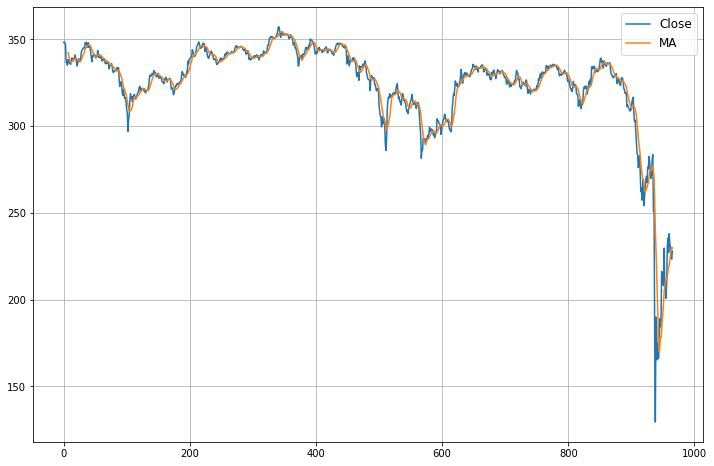
\includegraphics[scale=0.5]{MA_full.png}
  \caption{Скользящее среднее на всем диапазоне}
  \label{fig:MA_full}
\end{figure}

\begin{figure}[H]
  \centering
  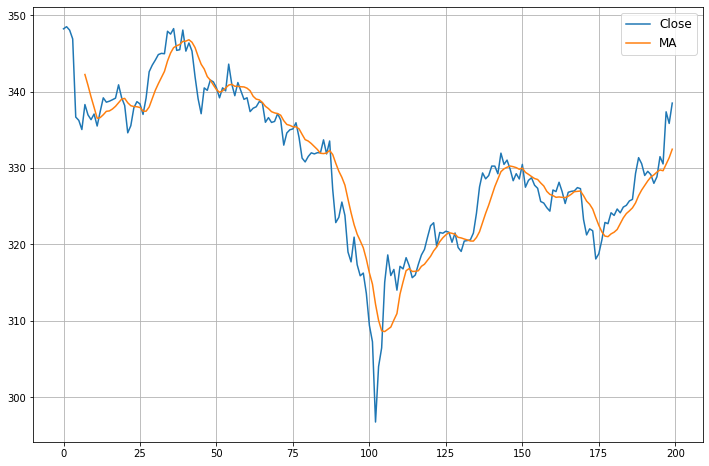
\includegraphics[scale=0.5]{MA_1.png}
  \caption{Скользящее среднее в диапазоне [:200]}
  \label{fig:MA_1}
\end{figure}

\begin{figure}[H]
  \centering
  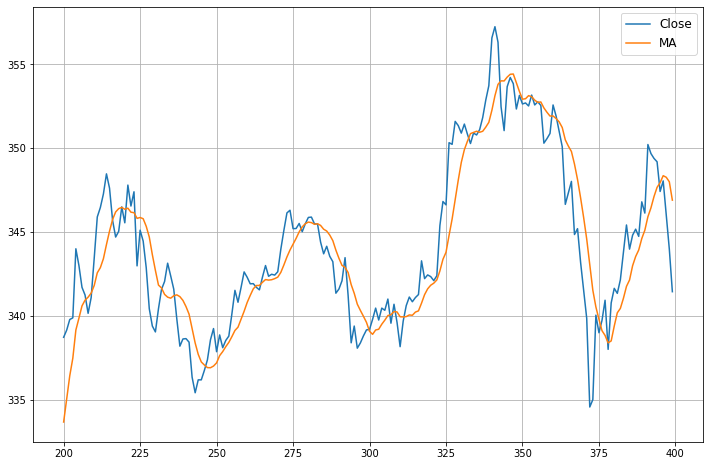
\includegraphics[scale=0.5]{MA_2.png}
  \caption{Скользящее среднее в диапазоне [200:400]}
  \label{fig:MA_2}
\end{figure}

\begin{figure}[H]
  \centering
  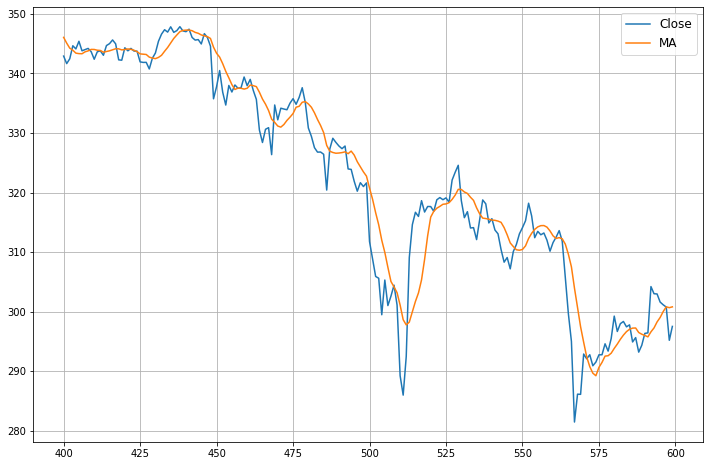
\includegraphics[scale=0.5]{MA_3.png}
  \caption{Скользящее среднее в диапазоне [400:600]}
  \label{fig:MA_3}
\end{figure}

\begin{figure}[H]
  \centering
  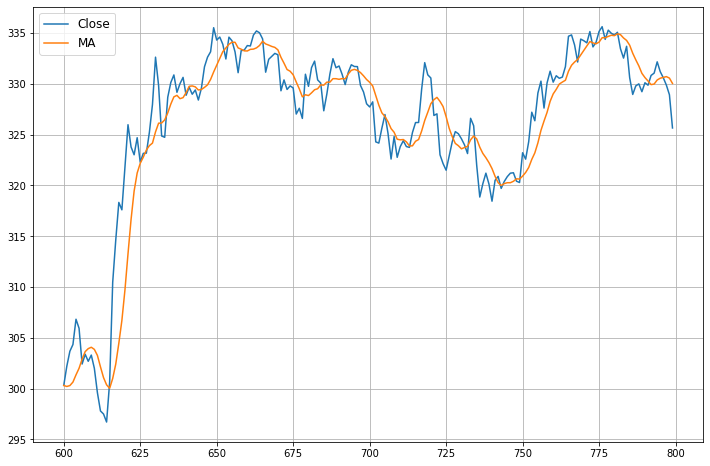
\includegraphics[scale=0.5]{MA_4.png}
  \caption{Скользящее среднее в диапазоне [600:800]}
  \label{fig:MA_4}
\end{figure}

\begin{figure}[H]
  \centering
  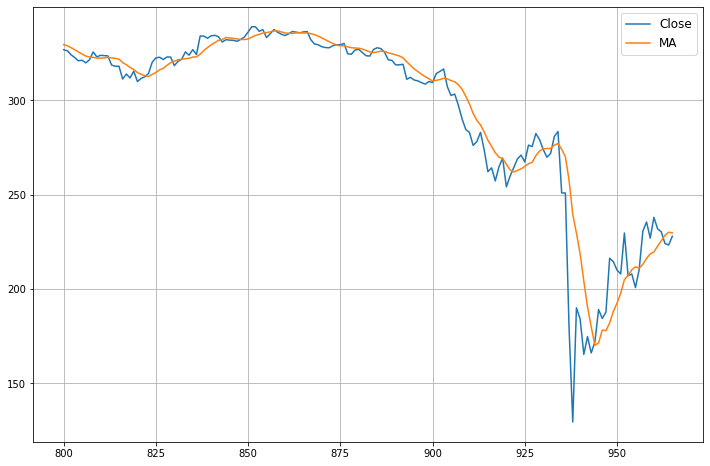
\includegraphics[scale=0.5]{MA_5.png}
  \caption{Скользящее среднее в диапазоне [800:]}
  \label{fig:MA_5}
\end{figure}

\pagebreak

Написана программы моделирующие сигналы на покупку и продажу.

\begin{lstlisting}[basicstyle=\small, language=Python]
  over_average = True
  bought = 0
  sold = 0

  def f_1(row):
      global over_average
      global bought
      global sold

      # up to down, sell
      # if more shares are bought than sold
      if over_average and row.close <= row.mov_avg and bought > sold:
          sold += 1
          over_average = row.close > row.mov_avg
          return row.close

      # down to up, buy
      elif not over_average and row.close >= row.mov_avg:
          bought += 1
          over_average = row.close > row.mov_avg
          return -row.close

      over_average = row.close > row.mov_avg

  print(
    df_moving_average[["close", "mov_avg"]] \
    .apply(f_1, axis=1) \
    .sum()
  )
  print(bought)
  print(sold)
\end{lstlisting}

Профит: 6.91 у.е.

Куплено 94 акции, продано 94 акции.

Эффективность вложенных средств: $6.91 / 100 = 0.0691$

\pagebreak

Стратегия генерации сигналов на покупку и продажу с использованием
скользящего среднего модифицирована, используется взвешенное среднее
с большим окном.

\[
  WMA = \frac{\sum_{i=1}^{n}w_i \cdot c_i}{\sum_{i=1}^{n}w_i}
\]
где $w: [1,n]$ - веса, а $c$ - текущее окно.

Размер окна выбран 9.

\begin{lstlisting}[basicstyle=\small, language=Python]
window_size_wma = 9
weights = np.arange(1, window_size_wma + 1)

df_moving_average['wma'] = df_moving_average.close\
  .rolling(window_size_wma)\
  .apply(lambda x: np.sum(weights*x)/np.sum(weights))

over_average = True
bought = 0
sold = 0

def f_2(row):
  global over_average
  global bought
  global sold

  # up to down, sell
  # if more shares are bought than sold
  if over_average and row.close <= row.wma and bought > sold:
      sold += 1
      over_average = row.close > row.wma
      return row.close

  # down to up, buy
  elif not over_average and row.close >= row.wma:
      bought += 1
      over_average = row.close > row.wma
      return -row.close

  over_average = row.close > row.wma

print(
  df_moving_average[["close", "wma"]]\
    .apply(f_2, axis=1)\
    .sum()
)
print(bought)
print(sold)
\end{lstlisting}

Профит: 11.67 у.е.

Куплено 103 акции, продано 103 акции.

Эффективность вложенных средств: $11.67 / 100 = 0.1167$

Эффективность возрасла в 1.69 раз.
\pagebreak

\subsection{Индекс силы (Force Index)}

Импорт данных (табл. \ref{table:data_per_day}):

\begin{lstlisting}[basicstyle=\small, language=Python]
  import pandas as pd

  df_force_index = pd \
    .read_csv('GAZP_211205_220305_per_day.csv', sep=";") \
    .rename(columns=lambda name: name[1:-1].lower())
\end{lstlisting}

\begin{table}[H]
  \centering
  \begin{tabular}{lllrr}
    \toprule
    {} & ticker &      date &   close &       vol \\
    \midrule
    0 &   GAZP &  06/12/21 &  338.94 &  70924550 \\
    1 &   GAZP &  07/12/21 &  344.96 &  75507480 \\
    2 &   GAZP &  08/12/21 &  340.50 &  78321390 \\
    3 &   GAZP &  09/12/21 &  336.60 &  61406510 \\
    4 &   GAZP &  10/12/21 &  332.00 &  44642520 \\
    ... &   ... &  ... &  ... &  ... \\
    52 &   GAZP &  18/02/22 &  309.48 &  125452970 \\
    53 &   GAZP &  21/02/22 &  257.30 &  413243360 \\
    54 &   GAZP &  22/02/22 &  283.51 &  324922990 \\
    55 &   GAZP &  24/02/22 &  210.00 &  413550130 \\
    56 &   GAZP &  25/02/22 &  228.00 &  211877250 \\
    \bottomrule
  \end{tabular}
  \caption{Дневная стоимость акций Газпром АО}
  \label{table:data_per_day}
\end{table}

Подсчет индекса силы.

\begin{lstlisting}[basicstyle=\small, language=Python]
  df_force_index["force"] = \
    df_force_index.vol * df_force_index.close.diff(1)
\end{lstlisting}

Значение индекса силы отображено в таблице \ref{table:data_per_day_FI},
первый ряд значений отброшен, поскольку для него не определено значение индекса силы.

\begin{table}[H]
  \centering
  \begin{tabular}{lllrrr}
    \toprule
    {} & ticker &      date &   close &        vol &         force \\
    \midrule
    1 &   GAZP &  07/12/21 &  344.96 &   75507480 &  4.545550e+08 \\
    2 &   GAZP &  08/12/21 &  340.50 &   78321390 & -3.493134e+08 \\
    3 &   GAZP &  09/12/21 &  336.60 &   61406510 & -2.394854e+08 \\
    4 &   GAZP &  10/12/21 &  332.00 &   44642520 & -2.053556e+08 \\
    5 &   GAZP &  13/12/21 &  307.26 &  140577980 & -3.477899e+09 \\
    ... &   ... &  ... &  ... &  ... & ... \\
    52 &   GAZP &  18/02/22 &  309.48 &  125452970 & -1.760105e+09 \\
    53 &   GAZP &  21/02/22 &  257.30 &  413243360 & -2.156304e+10 \\
    54 &   GAZP &  22/02/22 &  283.51 &  324922990 &  8.516232e+09 \\
    55 &   GAZP &  24/02/22 &  210.00 &  413550130 & -3.040007e+10 \\
    56 &   GAZP &  25/02/22 &  228.00 &  211877250 &  3.813790e+09 \\
    \bottomrule
  \end{tabular}
  \caption{Индекс силы}
  \label{table:data_per_day_FI}
\end{table}

Подсчитано экспоненциальное скользящее среднее индекса силы с окнами 2 и 13.
\[ K = 2 / (window + 1) \]
\[ fi\_ema_{window}[window] = fi[window] \cdot K - fi\_ma[window - 1] \cdot (1 - K) \]
\[ fi\_ema_{window}[i] = fi[i] \cdot K - fi\_ema_{window}[i - 1] \cdot (1 - K) \]
где, $fi$ -- индекс силы, $fi\_ma$ -- скользящее среднее индекса силы,
$fi\_ema_{window}$ -- экспоненциальное среднее индекса силы с окном \textit{window}.

\begin{lstlisting}
  df_force_index["fi_ema2"]\
    = df_force_index.force\
      .ewm(min_periods=2, span=2, adjust=False).mean()

  df_force_index["fi_ema13"]\
    = df_force_index.force\
      .ewm(min_periods=13, span=13, adjust=False).mean()
\end{lstlisting}

\begin{table}[H]
  \centering
  \begin{tabular}{lllrrrrr}
    \toprule
    {} & ticker &      date &   close &       vol &        force &       fi\_ema2 &      fi\_ema13 \\
    \midrule
    13 &   GAZP &  23/12/21 &  339.81 &  72129000 & -4.140e+8 & -7.249e+07 &  1.610e+08 \\
    14 &   GAZP &  24/12/21 &  338.79 &  39005950 & -3.978e+7 & -5.068e+07 &  1.323e+08 \\
    15 &   GAZP &  27/12/21 &  343.97 &  29925890 &  1.550e+9 &  8.644e+07 &  1.356e+08 \\
    16 &   GAZP &  28/12/21 &  343.23 &  34848840 & -2.578e+8 &  1.162e+07 &  1.125e+08 \\
    17 &   GAZP &  29/12/21 &  340.33 &  43005060 & -1.247e+9 & -7.926e+07 &  7.865e+07 \\
    ... &   ... &  ... &  ... &  ... & ... & ... &  ... \\
    52 &   GAZP &  18/02/22 &  309.48 &  125452970 & -1.760e+09 & -1.423e+09 & -2.838e+08 \\
    53 &   GAZP &  21/02/22 &  257.30 &  413243360 & -2.156e+10 & -1.484e+10 & -3.323e+09 \\
    54 &   GAZP &  22/02/22 &  283.51 &  324922990 &  8.516e+09 &  7.275e+08 & -1.632e+09 \\
    55 &   GAZP &  24/02/22 &  210.00 &  413550130 & -3.040e+10 & -2.002e+10 & -5.741e+09 \\
    56 &   GAZP &  25/02/22 &  228.00 &  211877250 &  3.813e+09 & -4.132e+09 & -4.376e+09 \\
    \bottomrule
    \end{tabular}
  \caption{Скользящее экспоненциальное среднее индекса силы}
  \label{table:data_per_day_FI_EMA}
\end{table}

\vspace{.5cm}

Значение экспоненциального скользящего среднего индекса силы с окном 2 и 13
отображено в таблице \ref{table:data_per_day_FI_EMA} (поля fi\_ema2 и fi\_ema13 соотв.).
Первые 13 значений отброшены, поскольку для них не определены значения ИС:13-ЭСС.

График полученного экспоненциального скользящего среднего индекса силы
отображен на рисунке \ref{fig:FI_EMA_full}.
Также изображены графики для каждых 35 значений для наглядности
(рис. \ref{fig:FI_EMA_1}, \ref{fig:FI_EMA_2})

\begin{figure}[H]
  \centering
  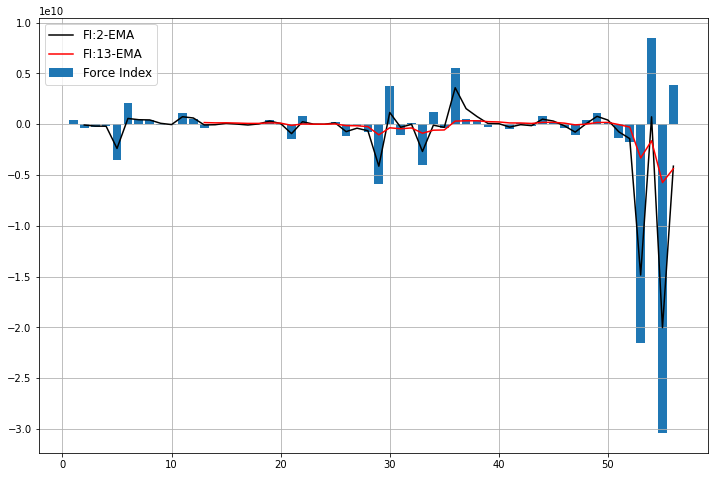
\includegraphics[scale=0.5]{FI_EMA_full.png}
  \caption{Скользящее экспоненциальное среднее индекса силы на всем диапазоне}
  \label{fig:FI_EMA_full}
\end{figure}

\begin{figure}[H]
  \centering
  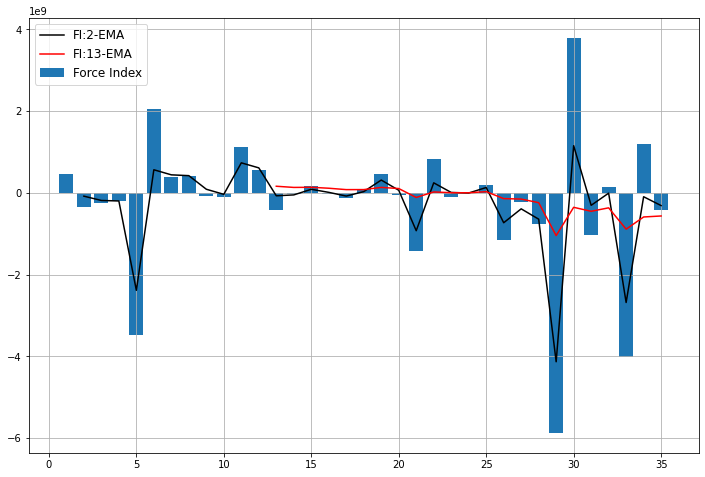
\includegraphics[scale=0.5]{FI_EMA_1.png}
  \caption{Скользящее экспоненциальное среднее индекса силы в диапазоне [:35]}
  \label{fig:FI_EMA_1}
\end{figure}

\begin{figure}[H]
  \centering
  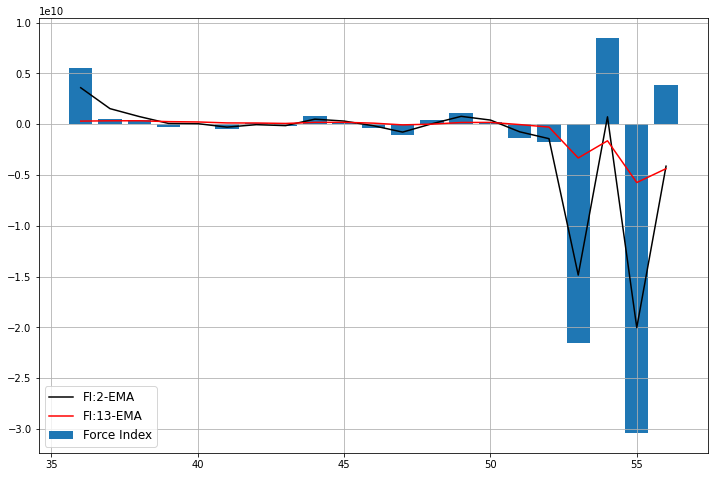
\includegraphics[scale=0.5]{FI_EMA_2.png}
  \caption{Скользящее экспоненциальное среднее индекса силы в диапазоне [35:]}
  \label{fig:FI_EMA_2}
\end{figure}


Написана программа моделирующая сигналы на покупку и продажу.
\begin{lstlisting}[basicstyle=\small, language=Python]
bought = []
sold = []

def ema_f(row):
    global bought
    global sold

    # buy
    if row.fi_ema2 < 0 and row.fi_ema13 > 0:
        bought.append(row.name)
        return -row.close
    
    # sell
    elif row.fi_ema2 > 0 and row.fi_ema13 < 0 and len(bought) > len(sold):
        sold.append(row.name)
        return row.close

print(df_force_index[["date", "close", "fi_ema2", "fi_ema13"]]\
  .apply(ema_f, axis=1).sum())
print(df_force_index.date[bought])
print(df_force_index.date[sold])
\end{lstlisting}

Профит: -2059.33 у.е.

Куплено 8 акций:
% \vspace{}
\begin{itemize}
  \setlength{\parskip}{0pt}
  \setlength{\itemsep}{0pt plus 1pt}
  \item[] 13    23/12/21
  \item[] 14    24/12/21
  \item[] 17    29/12/21
  \item[] 24    11/01/22
  \item[] 41    03/02/22
  \item[] 42    04/02/22
  \item[] 43    07/02/22
  \item[] 46    10/02/22
\end{itemize}

Продано 2 акции.

\begin{itemize}
  \setlength{\parskip}{0pt}
  \setlength{\itemsep}{0pt plus 1pt}
  \item[] 30    19/01/22
  \item[] 54    22/02/22
\end{itemize}

На руках осталось 6 акций (стоимостью по 228): 1368.

Эффективность вложенных средств: $(1368 - 2059.33) / 100 = -6.9133$

\subsection{Фьючерсы на акции российских и иностранных эммитентов}

Выбран фьючерсный контракт GAZR-12.21. Спецификация представлена на рисунке
\ref{fig:GAZR-12.21-specs}.

\begin{itemize}
  \item На один ФК приходится 100 акций
  \item Дата экспирации 17.12.2021
\end{itemize}

\clearpage

На рисунке \ref{fig:GZZ1-plot} изображен график контракта GAZR-12.21.

\begin{figure}[H]
  \centering
  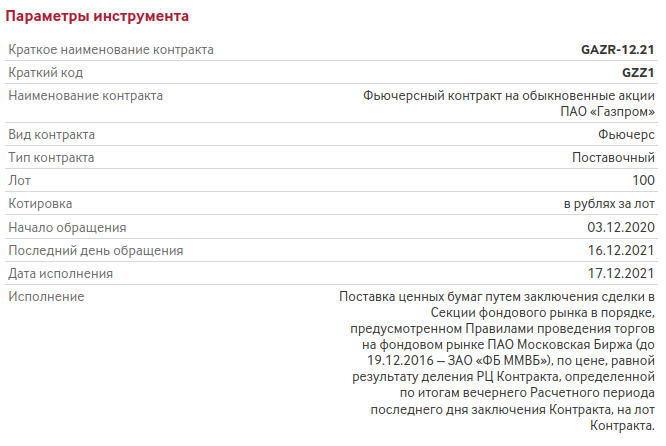
\includegraphics[scale=0.6]{specs.png}
  \caption{Спецификация контракта GAZR-12.21}
  \label{fig:GAZR-12.21-specs}
\end{figure}

\begin{figure}[H]
  \centering
  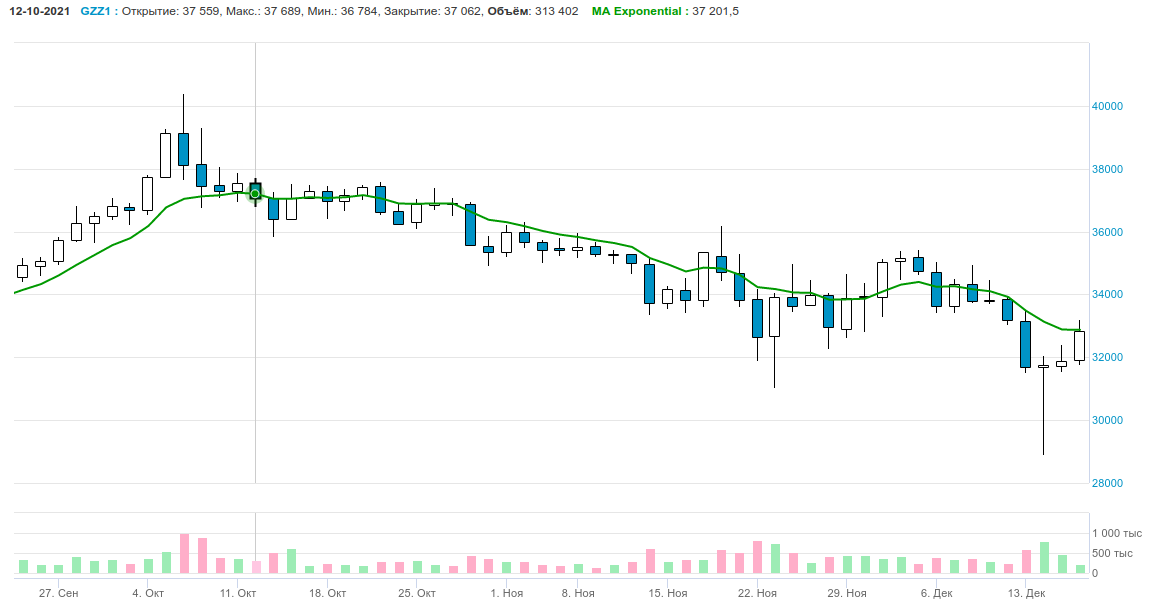
\includegraphics[scale=0.43]{GZZ1-plot.png}
  \caption{График контракта GAZR-12.21}
  \label{fig:GZZ1-plot}
\end{figure}

Первого сентября 2021 года куплено 100 акций ПАО Газпром по цене 312.89 за акцию.
Итого, потрачено 31289.

12 октября 2021 входим. Стоимость фьючерса превышает стоимость акций: 37062.

За день до экспирации, т.е. 16.12.2021 продаем акции и покупаем фьючерс.
Стоимость 100 акций: 32839. Стоимость фьючерса: 32850.

\begin{center}
  Прибыль $= 32839 - 31289 + 37062 - 32850 = 5762$
\end{center}


\section{Вывод}
В ходе выполнения работы изучены индикаторы технического анализа спотового рынка.

С помощью инструментальных средств смоделированы сигналы для покупки и продажи
акций на основе индикаторов скользящего среднего, и экспоненциального скользящего
среднего индекса силы.

Изучена стратегия купли-продажи фьючерсных контрактов. Принято решение,
обеспечившее прибыль.

\end{document}